\documentclass[paper]{ieicej}
%\documentclass[invited]{ieicej}% 招待論文
%\documentclass[survey]{ieicej}% サーベイ論文
%\documentclass[comment]{ieicej}% 解説論文
%\usepackage[dvips]{graphicx}
\usepackage[dvipdfmx]{graphicx,xcolor}
\usepackage[fleqn]{amsmath}
\usepackage{newtxtext}% 英数字フォントの設定を変更しないでください
\usepackage[varg]{newtxmath}% % 英数字フォントの設定を変更しないでください
\usepackage{latexsym}
%%図を二個横に並べるときに使用
\usepackage[hang,small,bf]{caption}
\usepackage[subrefformat=parens]{subcaption}
\usepackage{url}


\setcounter{page}{1}

\jtitle{VAEを用いた画像圧縮・異常検知を行う回路開発,\\及びエッジコンピューティングへの応用の検討}
\etitle{Implementation of a VAE-Based Circuit for Image Compression and Anomaly Detection \\and Its Potential Use in Edge Computing}


\authorlist{%
\authorentry[imamura.yuuki475@mail.kyutech.jp]{今村 優希}{Yuki Imamura}{kyutech}
\authorentry[kawasaki.taiga711@mail.kyutech.jp]{川崎 大雅}{Taiga Kawasaki}{kyutech}
% \authorentry[メールアドレス]{和文著者名}{英文著者名}{所属ラベル}
}
\affiliate[kyutech]{九州工業大学情報工学部 情報・通信工学科 3年\\ 福岡県飯塚市川津680-4}
  {Kyushu Institute of Technology, School of Computer Science and System Engineering, Department of Computer Science and Networks}
%\affiliate[所属ラベル]{和文勤務先\\ 連絡先住所}{英文勤務先\\ 英文連絡先住所}
\jalcdoi{???????????}% ← このままにしておいてください

\begin{document}
\begin{abstract}
%和文あらまし 500字以内
近年,無線通信技術の進化や5Gの普及が進んでおり,低遅延・多数同時接続の特性を活かした新たな通信環境の構築が求められている.
一方で,クラウド処理の負担増加による問題が考えられる.
これを解決する手法としてエッジコンピューティングが注目されている.
本研究では,エッジサーバー上での効率的なデータ処理を実現するため,VAEをFPGAを用いて実装し,取得した画像を圧縮・解析するシステムを開発した.
その結果,本システムにより画像圧縮と,異常検知を行うことができた.
しかし,落下物の色による判定精度の変動や処理速度の課題が残るため,より高精度なFPGAの活用やカラー画像の処理を取り入れることで,さらなる性能向上が期待される.
\end{abstract}
\begin{keyword}
%和文キーワード 4〜5語
VAE, FPGA, エッジコンピューティング
\end{keyword}
%\begin{eabstract}
%英文アブストラクト 100 words
%test
%\end{eabstract}
%\begin{ekeyword}
%英文キーワード
%VAE, FPGA, edge computing
%\end{ekeyword}
\maketitle

\section{はじめに}
近年,無線通信技術は飛躍的に向上しており,5G通信の普及が進んでいる.
5Gは従来の4Gなど通信規格と異なり,「高速大容量」「低遅延」「多数同時接続」の3つの特徴を備えており,その中でも「低遅延」と「多数同時接続」は新たな通信環境を構築する上で重要な軸となっている\cite{5g}.
従来の4G通信は,人が使用するスマートフォンや携帯に焦点を当てていた.
しかし,5Gでは車両,ドローン,センサなどのIoT機器が大量にネットワークに接続されることを前提としている.

また,今現在のIT業界ではクラウドが主流である\cite{jyotu-haku}.
図\ref{fig:1-1}の左側の処理のように,エッジデバイスからの処理をクラウドで実施し,その結果をエッジデバイスに通知するという仕組みである.
ただ,多くの端末から取得したデータをクラウドのみで処理を行うのはある程度限界があり,またトラヒック量が増加して,5Gのメリットを享受できないという問題が発生すると考えられる.

このような課題を解決するため,エッジコンピューティングという手法が近年注目され始めている.
エッジコンピューティングとは,従来はクラウドで行っていた処理の一部を,ユーザ端末(スマートフォンやIoT機器)の近い位置である基地局やその至近に設置されているサーバなどでデータ処理を行う技術である\cite{edge-com}\cite{nec-edge}.
この手法を用いることでクラウドにかかる処理をエッジコンピューティングで分散することが可能で,通信のトラヒック量の削減,5Gの特徴のひとつである「低遅延」を活用することも可能である.

\begin{figure}[tb]
  \begin{center}
    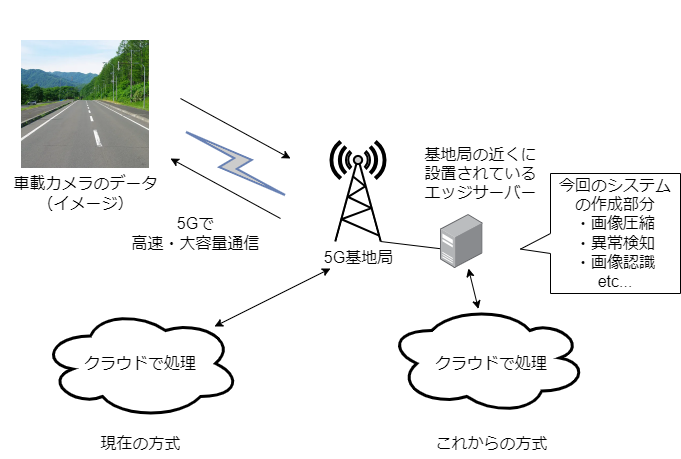
\includegraphics[width=0.98\columnwidth]{figures/Intr_1.png}
  \end{center}
  \caption{エッジコンピューティングのイメージと\\今回のシステムの作成部分}
  \label{fig:1-1}
\end{figure}

そこで,エッジコンピューティングの実現をVAEとFPGAを用いて実現することを考えた.
すでにVAEを用いて,道路上の異物を検知するシステムも作成されており,一定の成果を得ることができている\cite{vae-raod}.% 参考文献出す
したがって,今回は車載カメラから取得した画像をVAEを搭載したFPGAで処理を行い,図\ref{fig:1-1}の右側の処理の一部を作成することを目標とした.

\section{方法}
\subsection{実行環境}
今回のシステム作成において使用したツール及びそのバージョンを表\ref{tb:1}で示す.
また,FPGAの評価ボードとして,DIGILENT製のSoCを搭載したZYNQ-7010を使用する.

\begin{table}[tb]
  \centering
  \caption{使用したツール}
  \small
  \begin{tabular}{|c|c|} \hline
    用途 & 使用ツール \\ \hline \hline
    VAEシミュレーション用 & MATLAB 2024b \\ \hline
    ハードウェアシミュレーション & MATLAB/Simulink 2022a\\ \hline
    HDLコード生成 & HDL Coder \\ \hline
    FPGA設計ソフトウェア & Vivado 2022.1\\ \hline
    ハードウェアアクセラレーション & Vitis 2022.1 \\ \hline
    評価ボード & DIGILENT製 ZYNQ-7010 \\ \hline
  \end{tabular}
  \label{tb:1}
\end{table}


\subsection{システム構造}
今回のVAEを搭載したシステムでは,以下2つの機能を搭載した.
\begin{itemize}
  \item[1] 画像圧縮\\
  VAEの特徴のひとつである次元圧縮能力を画像に応用する.
  \item[2] 異常検知\\
  もう一つの特徴である異常検知を,元画像と生成画像とを比較して行う.  
\end{itemize}

全体の構想について解説する.
今回使用する画像は,簡単化のためにグレースケール化したものを使用する.
また,JPEGのようにブロックに分割して,それぞれのブロック毎にVAEを利用する.
ブロックサイズは$16\times16$に設定した.
ブロック毎に元画像と圧縮後の画像との比較はPSNRを用いて行う.
画像圧縮や異常検出はこのPSNRを用いて処理を行う.
画像圧縮では,PSNRが設定した閾値以上だった場合は,圧縮した潜在空間を用いても問題がないので,潜在空間を圧縮データとして利用する.
異常検知では,PSNRの値が閾値以下だった場合は道路以外の可能性が高いので異常と判定するよう設定する.

上記の機能を実現するために,VAEの構造を\ref{2.2.3}で説明する.
また,FPGAの構造の詳細を\ref{2.2.4}にて説明し,最後にSoC FPGAの構造を\ref{2.2.5}にて説明する.

\subsubsection{VAE構造}\label{2.2.3}
VAEの構造の概略を図\ref{fig:2-2-2-1}に示す.
$16×16$の画像を使用することから,入力256次元,出力256次元で設計を行った.
潜在空間の次元は,圧縮したとしてもある程度判別がつくように16次元で作成を行った.
エンコーダ部分の活性化関数に関しては,平均ではReLU関数を使用し,分散ではソフトプラス関数を使用している.
また,デコーダ部分ではシグモイド関数を利用している.
\begin{align}
  f(x) &= x &: ReLU関数\\
  f(x) &= \log(1+e^x) &: Softplus関数 \label{sq:2}\\
  f(x) &= \dfrac{1}{1+e^{-x}} &: Sigmoid関数 \label{sq:3}
\end{align}

また,VAEの学習方法を図\ref{fig:2-2-2-2}に示す.
まず,道路のみのブロックを大量に用意する.
そのブロックを教師データとし,VAEを学習させる.
学習の条件を表\ref{tb:2}にまとめた.
今回は道路が映った写真を用意し(図\ref{fig:2-2-2-2}の左上の画像),道路のみ映った部分(図\ref{fig:2-2-2-2}の右上の画像)をブロック化することで教師データの用意を行った.
また,MATLABでVAEの学習のみ行い,そこから出力された重みやパラメータを使用してFPGAに搭載したVAEの制御を行う.

\begin{table}[b]
  \centering
  \caption{学習条件}
  \small
  \begin{tabular}{|c|c|} \hline
    epoch & 10000 \\ \hline
    eta & 0.0005 \\ \hline
    Layer2(潜在空間の数) & 16 \\ \hline
  \end{tabular}
  \label{tb:2}
\end{table}


% VAEの構造図
\begin{figure}[tb]
  \begin{center}
    %Created by Kawasaki, Edited by Imamura
    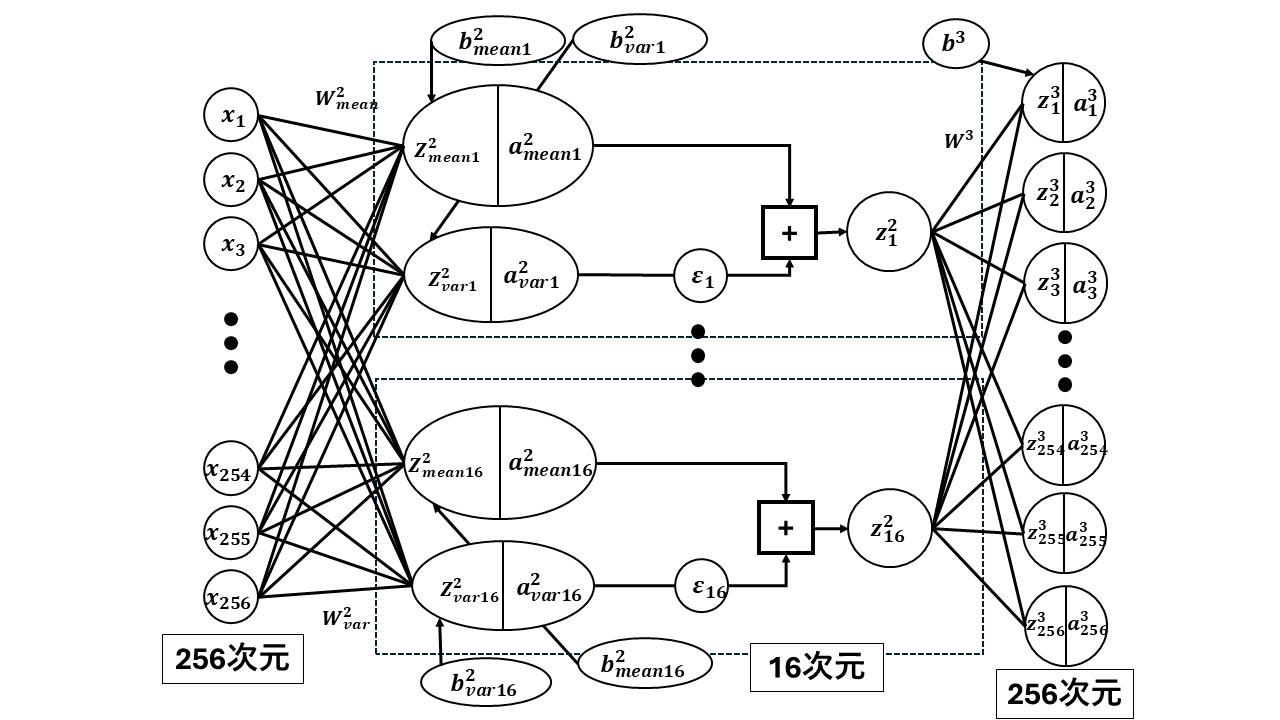
\includegraphics[width=0.98\columnwidth]{figures/VAE_1.png}
  \end{center}
  \caption{$256\times16\times256$VAEの構造}
  \label{fig:2-2-2-1}
\end{figure}

\begin{figure}[tb]
  \begin{center}
    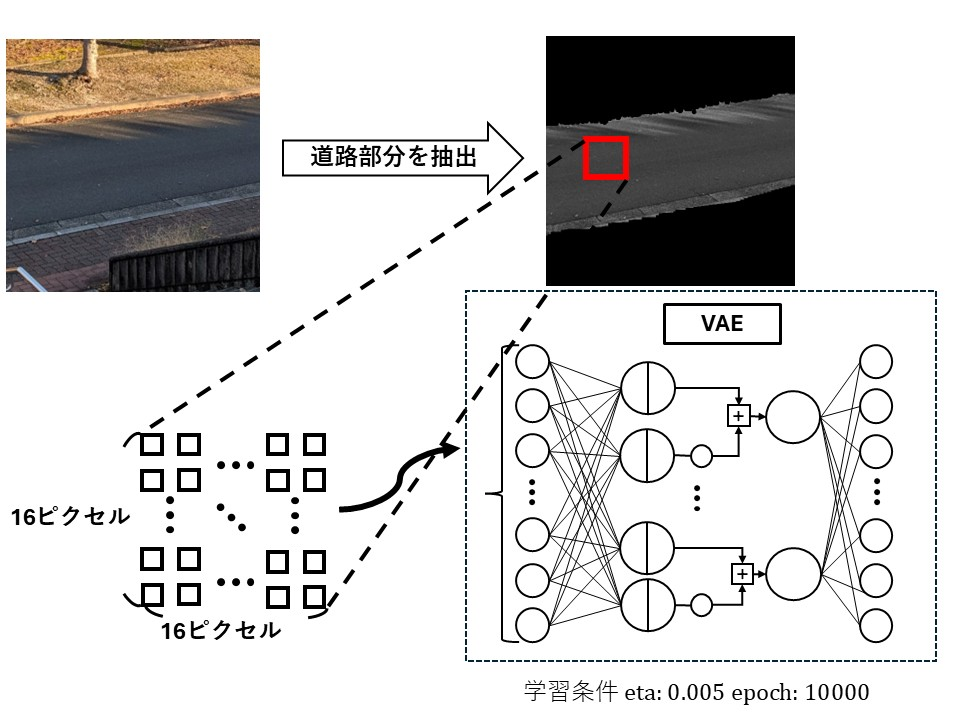
\includegraphics[width=0.98\columnwidth]{figures/VAE_2.jpg}
  \end{center}
  \caption{VAE学習方法}
  \label{fig:2-2-2-2}
\end{figure}

\subsubsection{FPGA構造}\label{2.2.4}
使用したボードは,DIGILENT製のZYNQ-7010である.
今回の設計では,図\ref{fig:2-2-3-1}に示すように,入力データとして,$X(16)$,$W(16\times2)$,$b(16)$,出力として$Z(16)$を用意した(()内は次元数).
赤色の枠で囲われているユニットは出力を$Output_1$とすると,
\begin{align}
  Output_1 = X_1 \times W1_1
\end{align}
のような,入力と重みのパラメータを乗算する演算を行っている.
その演算ユニットを16個用意したものが,青色の枠線で囲われているユニットである.
最終的な一つの$Z$の出力は,
\begin{align}
  Z_1 = \sum_{i = 0}^{16} X_i \times W1_i + b1
\end{align}
の計算を行っている.

当初は入力256,出力256の演算をFPGAに載せたかったが,容量に限界があった.
したがって,今回設計した$256\times16\times256$のVAEを実現しやすい,$X$の入力が16になるように設計を行った.

% FPGA内の構造図
% エンコーダの中身
\begin{figure}[tb]
  \begin{center}
    %入力画像はPNG
    %created by Imamura
    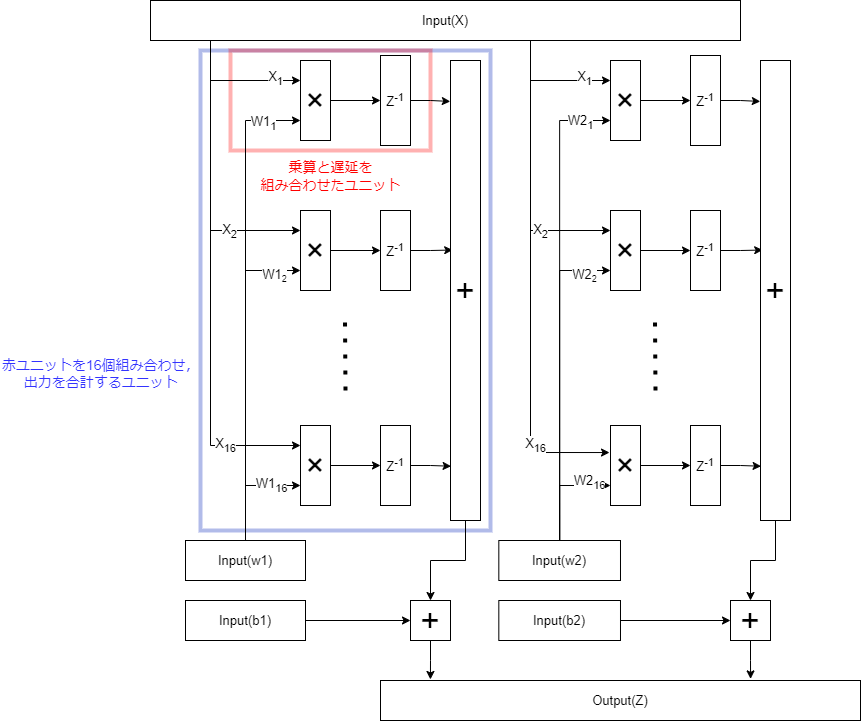
\includegraphics[width=0.98\columnwidth]{figures/FPGA_1.png}
  \end{center}
  \caption{FPGAの構造}
  \label{fig:2-2-3-1}
\end{figure}

\subsubsection{SoC FPGAの構造}\label{2.2.5}
SoC FPGAのシステム構造の概要を図\ref{fig:2-2-4-1}にて示す.
\texttt{processing\_system7\_0}がバスを通って様々な処理を行っおり,CPUの役割を担っている.
また,\texttt{dut\_forwa\_ip\_0}の部分が今回作成したFPGAの部分である.
実装した後のリソース利用評価を表\ref{tb:3}に示す.

次に,SoC FPGAの処理の概要を図\ref{fig:2-2-4-2}にて示す.
SDカードには,CSVファイルに格納した重みやパラメータ,RAW形式の画像データが格納されている.
それらのデータをCPUが読み取る.
その後,作成したFPGAに従って入力データの処理を行い,FPGAにそのデータを送信する.
FPGAはデータが格納されると同時に実行し,出力結果を保存する.
その出力結果をCPUが読み取りに行き,出力データを処理する.
それらの処理を繰り返し行う.

今回のVAEが$256\times16\times256$であり,\ref{2.2.4}で作成したFPGAの構造が$16\times2$である.
設計したFPGAを一回稼働させることで処理できる部分を図\ref{fig:2-2-4-3}に示す.
エンコーダでは,2つの出力の計算を$z^2_{mean}$,$z^2_{var}$にあてる.
一回の使用で,256次元の入力のうち16次元処理できるので,1つの潜在空間を計算させるためにはFPGAを16回使用する必要がある.
出力された$z^2_{mean}$,$z^2_{var}$を$b$に格納するよう設計をした.
その潜在空間が16個あるので,エンコーダの計算は合計で$16\times16=256$回稼働する.
デコーダ部分を計算する際は,FPGAを一回稼働させるだけで,3層目$Z^3_i$の出力256次元のうち2次元の結果を得られる.
したがって,デコーダでは128回FPGAを稼働させる.
このような制御をCPUで作成した.

出力で得た$z^2_{mean}$,$z^2_{var}$,$z^3$は,ソフトウェア上で活性関数を用いて$a^2_{mean}$,$a^2_{var}$,$a^3$の計算を行う.
さらに,$a^2_{mean}$と$a^2_{var}$を用いて$z^2$の計算もソフトウェア上で行っている.
最後に,入力画像と出力の$a^3$の値を比較し,PSNRを計測を行っている.

\begin{table}[tb]
  \centering
  \caption{FPGAのリソース利用率}
  \small
  \begin{tabular}{|c|c|c|c|} \hline
    Resorce & Utilization & Available & Utilization[\%]\\ \hline
    LUT & 3301 & 17600 & 18.76 \\ \hline
    LUTRAM & 62 & 6000 & 1.03 \\ \hline
    FF & 3297 & 35200 & 9.37 \\ \hline
    DSP & 64 & 80 & 80.0 \\ \hline
    IO & 12 & 100 & 12.0 \\ \hline
    BUFG & 1 & 32 & 3.13 \\ \hline
  \end{tabular}
  \label{tb:3}
\end{table}

% SoC構造図
\begin{figure}[tb]
  \begin{center}
    %created by screenshot
    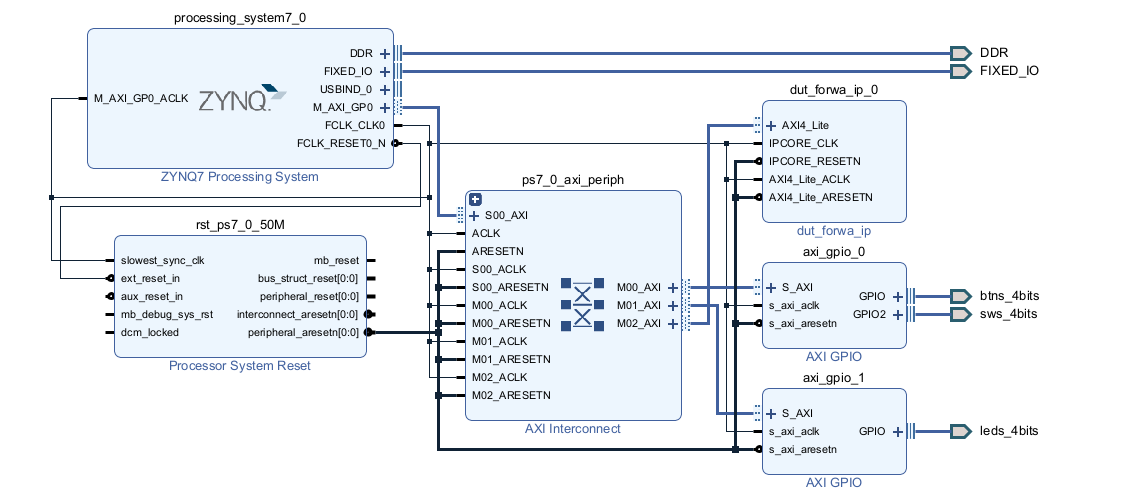
\includegraphics[width=0.98\columnwidth]{figures/SoC_1.png}
  \end{center}
  \caption{SoC FPGAの構成図}
  \label{fig:2-2-4-1}
\end{figure}

\begin{figure}[tb]
  \begin{center}
    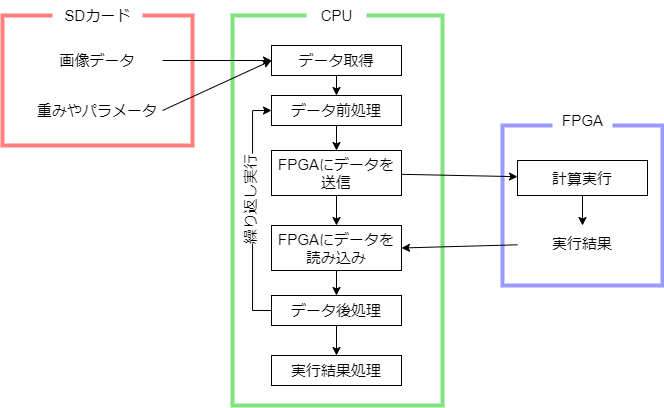
\includegraphics[width=0.98\columnwidth]{figures/SoC_2.png}
  \end{center}
  \caption{SoC FPGAの処理概要}
  \label{fig:2-2-4-2}
\end{figure}

\begin{figure}[tb]
  \begin{center}
    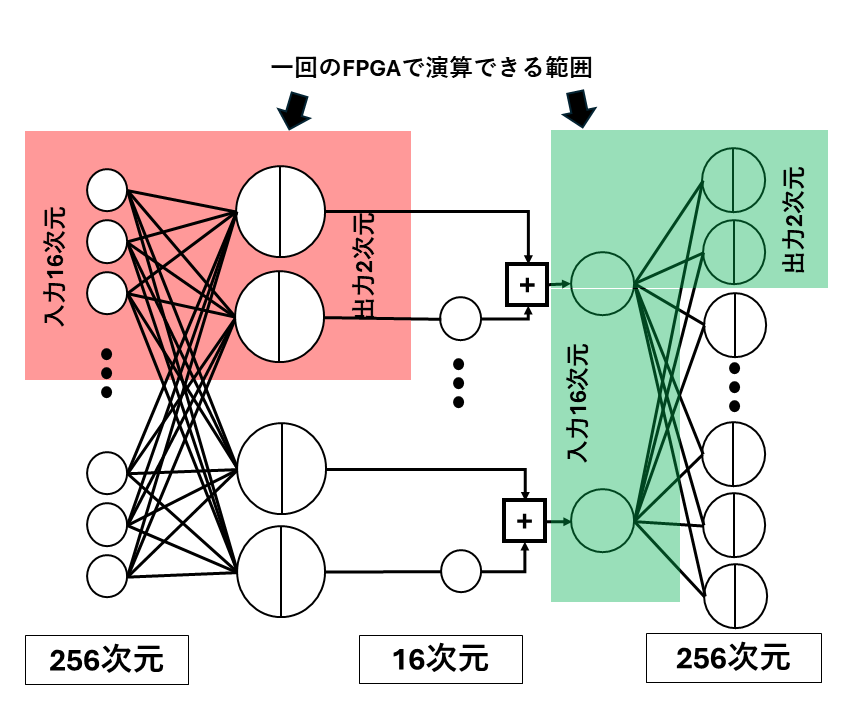
\includegraphics[width=0.98\columnwidth]{figures/SoC_3.png}
  \end{center}
  \caption{FPGAの利用イメージ}
  \label{fig:2-2-4-3}
\end{figure}

\subsection{実験方法}
今回は,図\ref{fig:2-3-1}に示す3種類の画像を用意した.
図\ref{fig:2-3-2}は,落下物がない画像である.
図\ref{fig:2-3-3}と図\ref{fig:2-3-4}は,落下物があるのをイメージしたものであり,異常検知の比較を行うために用意した.
画像のサイズは$512\times512$で,VAEに通す際は,画像をグレー画像にしている.
$16\times16$のブロックで分割をしながら処理を行い,PSNRを計測する.
そのPSNRがMATLABの出力とFPGAを用いた出力でどの程度の差があるのかを比較する.
FPGAで出力されたPSNRはCSVファイルに書き込み,そのデータをMATLAB上で提示する.

\begin{figure}[tb]
  \begin{minipage}[]{0.32\columnwidth}
    \centering
    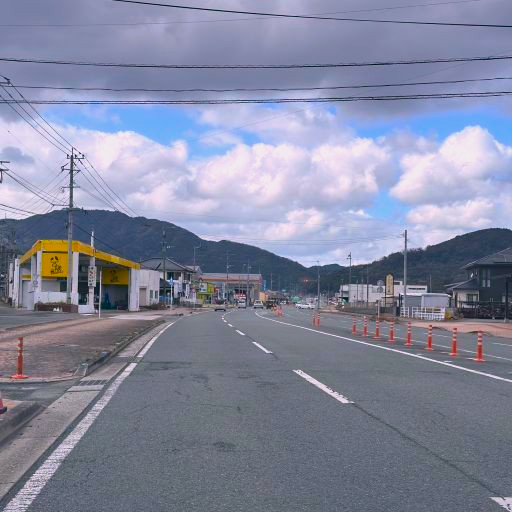
\includegraphics[width=0.9\columnwidth]{figures/Ex_pr1.png}
    \subcaption{画像1\\もともとの画像}
    \label{fig:2-3-2}
  \end{minipage}
  \begin{minipage}[]{0.32\linewidth}
    \centering
    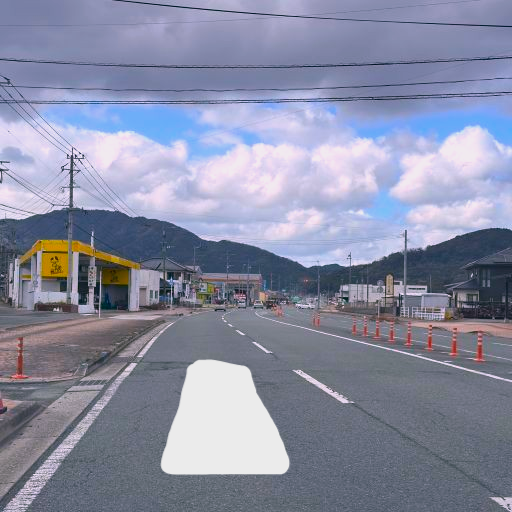
\includegraphics[width=0.9\columnwidth]{figures/Ex_pr2.png}
    \subcaption{画像2\\落下物がある画像}
    \label{fig:2-3-3}
  \end{minipage}
  \begin{minipage}[]{0.32\linewidth}
    \centering
    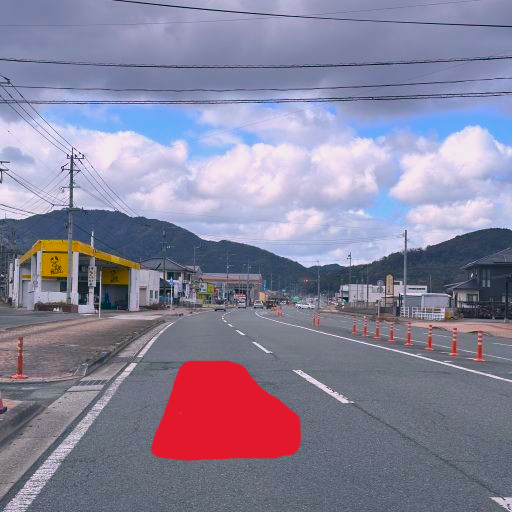
\includegraphics[width=0.9\columnwidth]{figures/Ex_pr3.png}
    \subcaption{画像3\\落下物がある画像}
    \label{fig:2-3-4}
  \end{minipage}
  \caption{今回テストする評価画像}
  \label{fig:2-3-1}
\end{figure}

\section{実験と考察}
\subsection{実験結果}
まず,SoC FPGAの実行画面を図\ref{fig:3-1}に示す.
ボタン0を押すことでSDカードに保存されているCSVファイルを読み込んでいる.
ボタン1から3で画像をVAEに通過させる処理を行っている.
図\ref{fig:3-1}はボタン0を押し,パラメータを取得後の状態である.

\begin{figure}
  \begin{center}
    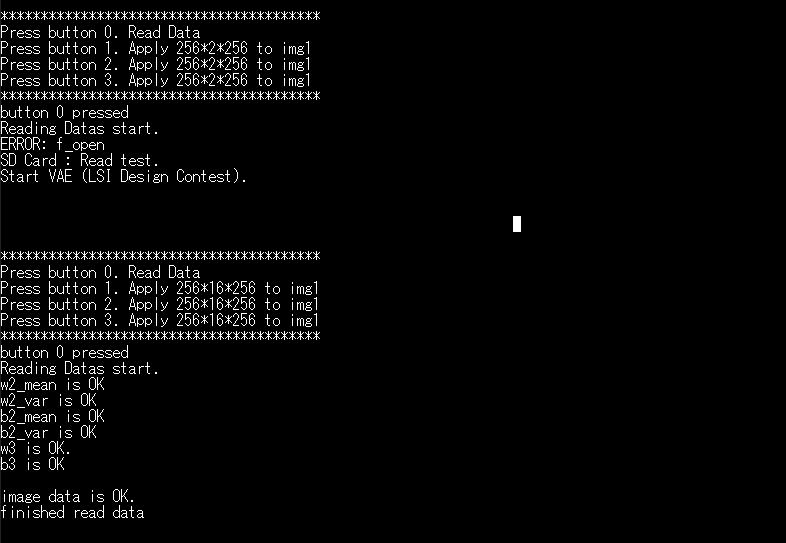
\includegraphics[width=0.98\columnwidth]{figures/Ex_re7.png}
  \end{center}
  \caption{SoC FPGAの実行画面}
  \label{fig:3-1}
\end{figure}


\subsubsection{画像1(図\ref{fig:2-3-2})の出力比較}
図\ref{fig:3-1-3}にMATLABでの出力,図\ref{fig:3-1-4}にFPGAでの出力を示す.
MATLABでは道路の部分付近のPSNRが25以上の値を示していることがわかる.
加えて,空や山の一部分もPSNRが高くなっている.
FPGAの出力では,MATLABと比較して全体的にPSNRが低くなっていることがわかる.
ただ,道路部分のPSNRは25程度と,結果としては悪くない値を出している.
\begin{figure}[tb]
  \begin{minipage}[]{0.32\columnwidth}
    \centering
    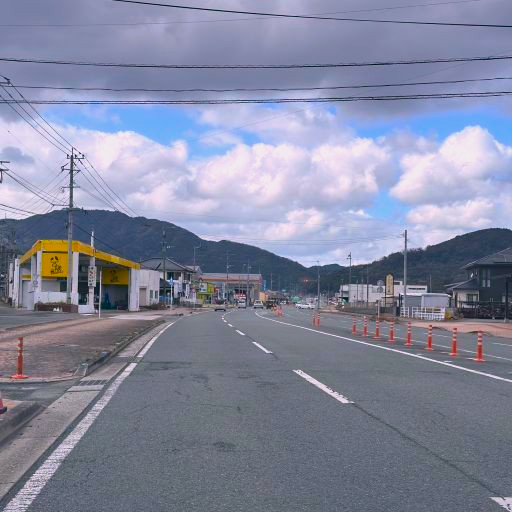
\includegraphics[width=0.9\columnwidth]{figures/Ex_pr1.png}
    \subcaption{テストする画像1}
    \label{fig:3-1-2}
  \end{minipage}
  \begin{minipage}[]{0.32\linewidth}
    \centering
    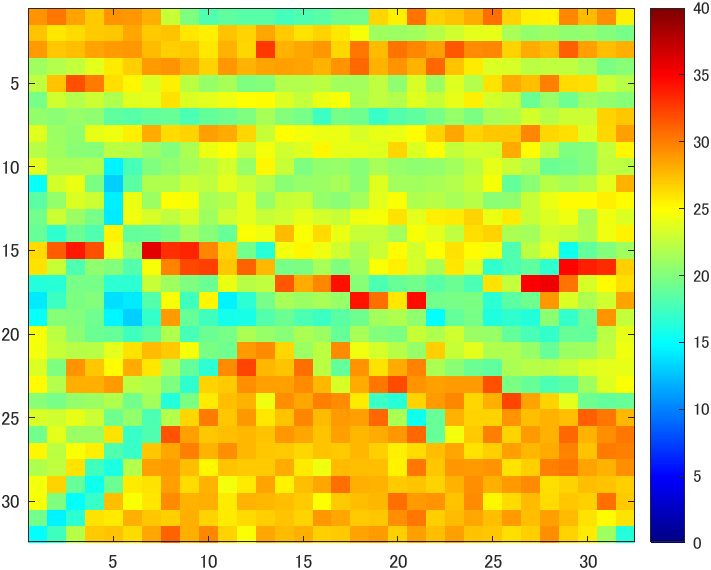
\includegraphics[width=0.9\columnwidth]{figures/Ex_re1.png}
    \subcaption{PSNRをブロック毎に出力\\MATLABでの出力}
    \label{fig:3-1-3}
  \end{minipage}
  \begin{minipage}[]{0.32\linewidth}
    \centering
    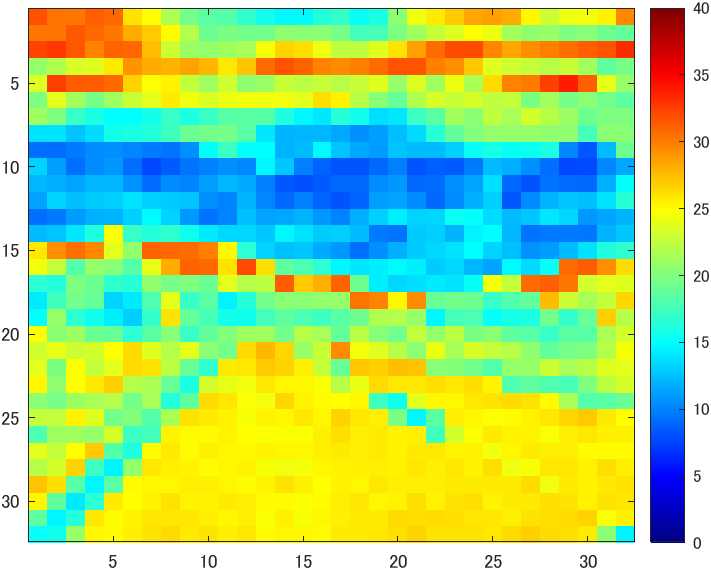
\includegraphics[width=0.9\columnwidth]{figures/Ex_re2.png}
    \subcaption{PSNRをブロック毎に出力\\FPGAでの出力}
    \label{fig:3-1-4}
  \end{minipage}
  \caption{画像1の処理結果}
  \label{fig:3-1-1}
\end{figure}

\subsubsection{画像2(図\ref{fig:2-3-3})の出力比較}
図\ref{fig:3-2-3}にMATLABでの出力,図\ref{fig:3-2-4}にFPGAでの出力を示す.
MATLAB.FPGAの出力双方とも落下物の部分のPSNRが悪化している.

\begin{figure}[tb]
  \begin{minipage}[]{0.32\columnwidth}
    \centering
    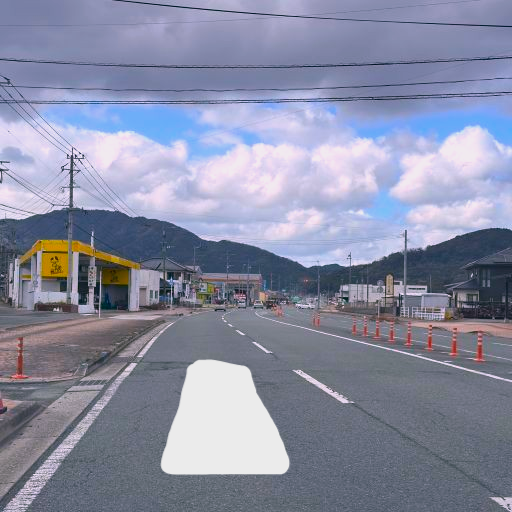
\includegraphics[width=0.9\columnwidth]{figures/Ex_pr2.png}
    \subcaption{テストする画像2}
    \label{fig:3-2-2}
  \end{minipage}
  \begin{minipage}[]{0.32\linewidth}
    \centering
    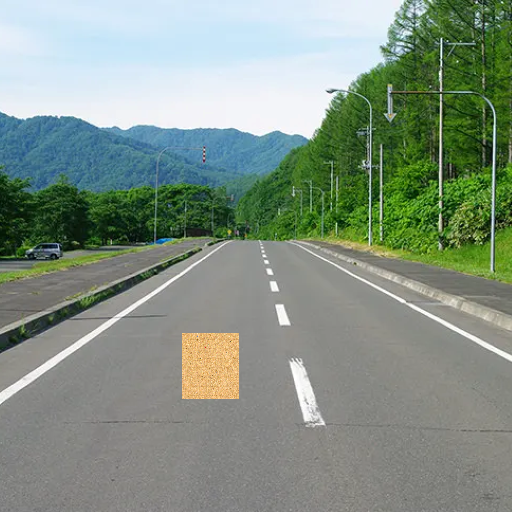
\includegraphics[width=0.9\columnwidth]{figures/Ex_re3.png}
    \subcaption{PSNRをブロック毎に出力\\MATLABでの出力}
    \label{fig:3-2-3}
  \end{minipage}
  \begin{minipage}[]{0.32\linewidth}
    \centering
    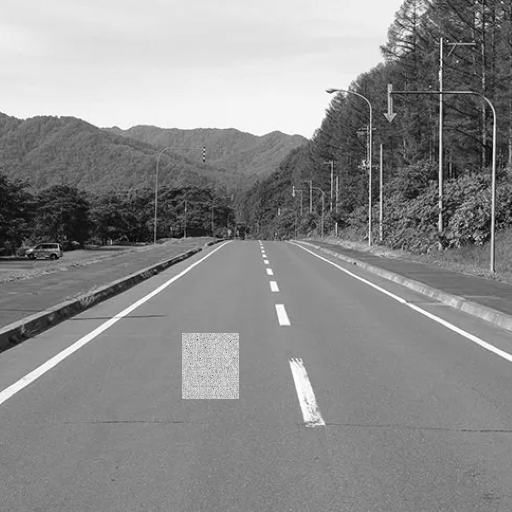
\includegraphics[width=0.9\columnwidth]{figures/Ex_re4.png}
    \subcaption{PSNRをブロック毎に出力\\FPGAでの出力}
    \label{fig:3-2-4}
  \end{minipage}
  \caption{画像2の処理結果}
  \label{fig:3-2-1}
\end{figure}

\subsubsection{画像3(図\ref{fig:2-3-4})の出力比較}
図\ref{fig:3-3-3}にMATLABでの出力,図\ref{fig:3-3-4}にFPGAでの出力を示す.
画像2の出力と異なり,逆に落下物がある部分のPSNRが向上している.

\begin{figure}[tb]
  \begin{minipage}[]{0.32\columnwidth}
    \centering
    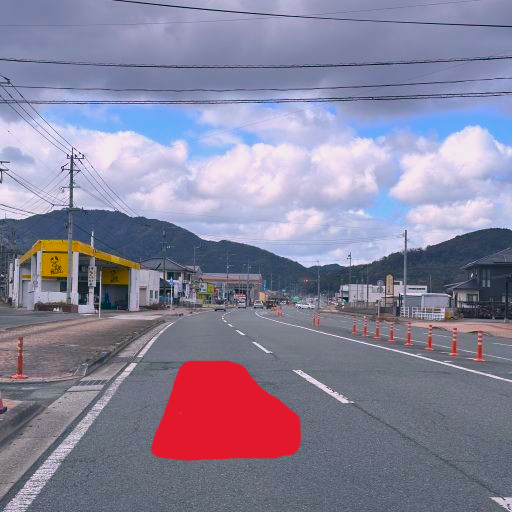
\includegraphics[width=0.9\columnwidth]{figures/Ex_pr3.png}
    \subcaption{テストする画像3}
    \label{fig:3-3-2}
  \end{minipage}
  \begin{minipage}[]{0.32\linewidth}
    \centering
    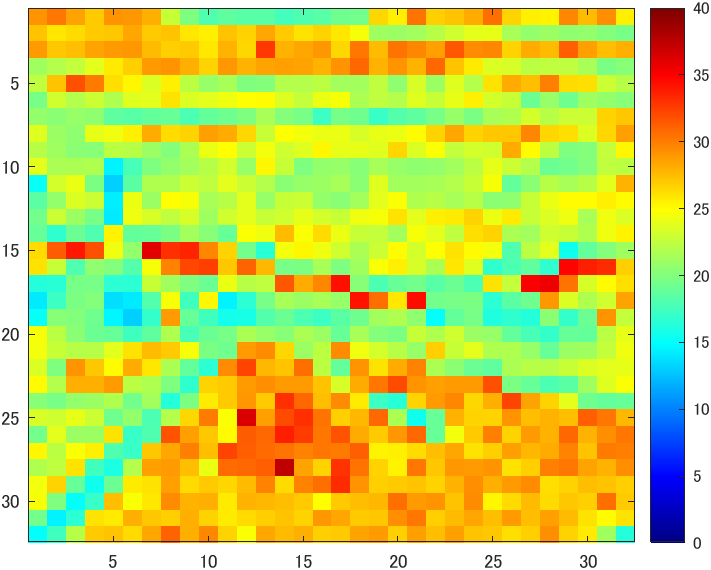
\includegraphics[width=0.9\columnwidth]{figures/Ex_re5.png}
    \subcaption{PSNRをブロック毎に出力\\MATLABでの出力}
    \label{fig:3-3-3}
  \end{minipage}
  \begin{minipage}[]{0.32\linewidth}
    \centering
    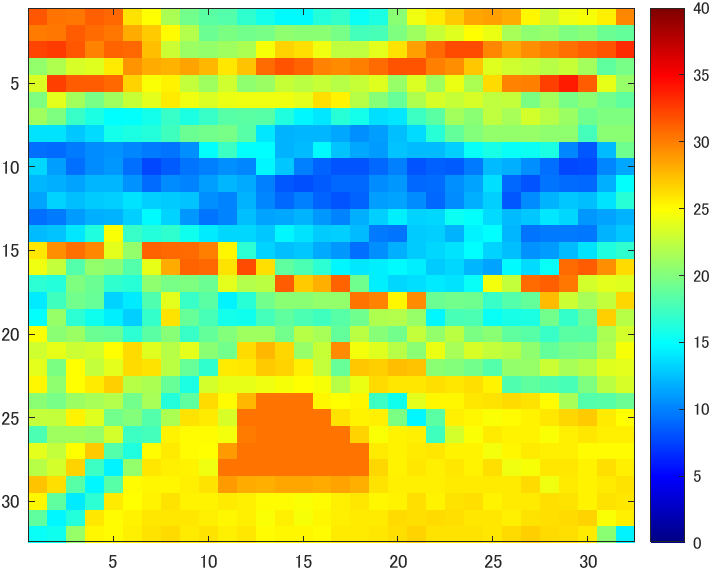
\includegraphics[width=0.9\columnwidth]{figures/Ex_re6.png}
    \subcaption{PSNRをブロック毎に出力\\FPGAでの出力}
    \label{fig:3-3-4}
  \end{minipage}
  \caption{画像3の処理結果}
  \label{fig:3-3-1}
\end{figure}

\subsubsection{結果まとめ}
それぞれの出力画像を比較して,MATLABとFPGAの出力結果には違いが見られた.
しかし,FPGAでも道路の部分が他の部分と比較してPSNRが高いため,失敗はしていないと考える.

また,異常検知に関しては,落下物の色に影響を受けることが発見された.
落下物が白であると,PSNRが悪化する一方で,赤色ではPSNRが向上するという結果が得られた.

\subsection{考察}
\subsubsection{全体}
得られた結果から,以下の3点で考察を行う.
\begin{enumerate}
  \item 道路以外もPSNRが高い点 \label{3-1-0}
  \item MATLABとFPGAの出力が異なる点 \label{3-1-1}
  \item 赤色の物体もPSNRが向上している点 \label{3-1-2}
\end{enumerate}

(\ref{3-1-0})に関しては,グレー化した影響とVAEの特性にるものと,2つの観点で考えられる.
特に,空の部分はグレースケール化すると,道路の部分のように特徴量が少ない.
したがって,今回作成したVAEでも表現が可能で,VAEの画像復元能力を発揮することができていると考えられる.

(\ref{3-1-1})に関しては,用いた変数や,固定小数点の誤差によって生じたと考えられる.
ただ,詳細の出力を確認できていないため,今後検証を行って原因究明を行っていく.

(\ref{3-1-2})に関しては,グレースケール化によって生じていると考えられる.
赤色をグレースケール化した際,道路の色の濃さとほぼ同じになっていた(図\ref{fig:3-3-5}).
このことから,正しく落下物を判定するためにはカラースケールで処理を行う必要があると考えられる.

\begin{figure}
  \begin{center}
    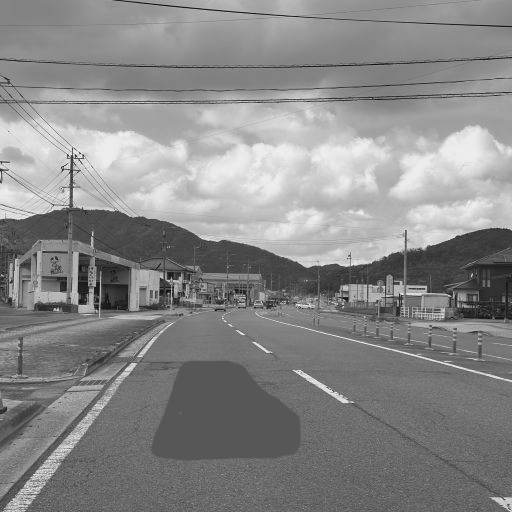
\includegraphics[width=0.45\columnwidth]{figures/De_re1.png}
  \end{center}
  \caption{画像3をグレースケールに変換した画像}
  \label{fig:3-3-5}
\end{figure}

\subsubsection{エッジコンピューティングでの採用の評価}
エッジコンピューティングとして採用できるかを評価する.

まずは,画像圧縮について評価する.
今回はPSNRの閾値を25とし,閾値以上を圧縮可能,それ未満を圧縮不可能として判定を行う.
閾値が25以上のブロック数,圧縮前の容量,圧縮後の容量,圧縮率を表\ref{tb:4}に示す.
サイズの計算を数式(\ref{sq:10})に示す.
元画像が0から255の値を取ることから1ピクセル8bitである.
また,潜在空間を圧縮データを用いるため,8bitの固定小数点数を使用するとする.
$B$は閾値以上のブロック数を示している.
\begin{align}
  size = B \cdot 16 \cdot 8[bit] + (32\cdot32 - B) \cdot 16 \cdot 16 \cdot 8[bit] \label{sq:10}
\end{align}
どの画像でも圧縮率が30\%近くの値を出せている.
圧縮した画像をクラウドに送信し,処理を行ってもらうことで,基地局から処理サーバーまでのトラヒック量の軽減や,クラウドでの処理速度を向上することができると考えられる.

\begin{table}[tb]
  \centering
  \caption{画像圧縮効果}
  \small
  \begin{tabular}{|c|c|c|c|c|} \hline
    画像 & ブロック数 & 圧縮前[bit] & 圧縮後[bit] & 圧縮率[\%]\\ \hline
    1 & 346 & 2097152 & 1432832 & 68.32 \\ \hline
    2 & 305 & 2097152 & 1511552 & 72.08 \\ \hline
    3 & 349 & 2097152 & 1427072 & 68.05 \\ \hline
  \end{tabular}
  \label{tb:4}
\end{table}

次に,異常検知について評価する.
実験結果でも示したように,落下物の色によって異常検知ができるかが変わる.
しかし,白色では異常検知が可能であることから,処理画像をカラー画像で行えば可能であると考えられる.
これから走行するであろう部分を認識対象に行うと,認識結果を即座に車両に通知することで事故の回避ができると考えられる.

最後に,エッジコンピューティングで重要なリアルタイム性を評価する.
一つの画像を入力し,PSNRを出力するのに,今回のシステムは4から5秒程度の時間を要した.
このままだと異常判定を行う前に事故が発生してしまいかねない.
処理に時間がかかった原因として,時間のかかるバスを用いてデータの書き込み・読み込みを何度も行ったからであると考えられる.
今回はFPGAに搭載できた回路は,VAEの一部分であり,何度もFPGAを実行しており,その度にバスを用いたデータ転送を行っている.
実際に$512\times512$の画像をVAEで処理を行うためには,FPGAを$393216$回動作させている.
ただ,より高精度なFPGAを用いることでこの問題も解決できる可能性は高い.

\section{結論と今後の展望}
今回は,VAEをFPGAを上に実装し,道路画像の圧縮及び異常検知を行うシステムを構築した.
その結果,FPGAを用いたエッジコンピューティングにおける画像処理が実現可能であることを示した.

本システムにはいくつかの課題があるものの,適切な改善により解決可能であると考える.
したがって,将来的な産業応用の可能性も秘めていると思う.

今回のコンテストでFPGAを用いたLSI開発を体験することができた.
FPGAの将来性を感じたし,AIが日常的に使用されている現在に計算を効率よく行うために必要なデバイスであることを認知した.
これからもFPGAの能力を発揮できるような開発を行っていきたいし,高位合成等のFPGAを開発するための技術も日々進化しているので,様々なことに挑戦していきたい.

\ack
今回のコンテスト開催をしてくださったLSIデザインコンテスト実行委員会,ならびに支援をしてくださった主催・共催・協賛・後援の各団体の皆様,ありがとうございました.
また,研究室にも配属されていないのに,様々な支援をして頂いた先生方,本当にありがとうございました.
%\bibliographystyle{sieicej}
%\bibliography{myrefs}
\begin{thebibliography}{99}% 文献数が10未満の時 {9}
\bibitem{5g} 
森川博之, 5G次世代移動通信規格の可能性, 岩波書店, 東京, 2020.
\bibitem{edge-com} 
田中裕也, 高橋紀之, 河村龍太郎, "IoT時代を拓くエッジコンピューティングの研究開発", NTT技法ジャーナル, vol.27, no.8, pp.59-63, 2015.
\bibitem{nec-edge}
横田治樹, 尾田眞也, 小林宰, 石井大二, 伊東孝紘, 五十棲 淳考, "IoTのミッシングリンクをつなぐエッジコンピューティング技術", NEC技法, Vol.70, No.1, 2017.
\bibitem{jyotu-haku}
総務省, "令和6年版情報通信白書", 2024.
\bibitem{vae-raod}
山本健生, 橋本敦史, 岡本大和, "平均画像に対するVAE異常検知の適用による道路落下物検出", 人工知能学会全国大会論文集, 第35回, 2021.
\bibitem{LSI}
"LSI Design Contest", \url{http://www.lsi-contest.com/}, 20250131閲覧.

\end{thebibliography}

\end{document}
